\documentclass [a4paper] {report}
\usepackage{amsmath,amssymb,amsthm, bbm, graphicx,listings,braket,subfig,titlesec,cleveref,lipsum,mcode,xcolor-patch, textcomp,float,booktabs,siunitx, listings}
\usepackage[authoryear]{natbib}
\usepackage[section]{placeins}
\usepackage[margin=2.2cm]{geometry}
\titleformat{\chapter}{\normalfont\huge}{\thechapter.}{20pt}{\huge \bf}

\DeclareMathOperator*{\argmin}{arg\,min}
\DeclareMathOperator*{\argmax}{arg\,max}
\newcommand{\norm}[1]{\left\lVert #1 \right\rVert}

\begin{document}
	
	\begin{titlepage}
		\begin{center}
			
			\textsc{\LARGE IN4320 Machine Learning}\\[1.25cm]
			
			\rule{\linewidth}{0.5mm}\\[1.0cm]
			{\huge \bfseries Final Assignment }\\[0.6cm]
			\rule{\linewidth}{0.5mm}\\[1.5cm]
			
			\begin{minipage}{0.4\textwidth}
				\begin{flushleft} \large	
					\emph{Author:}\\
					\textsc{Milan Niestijl, 4311728}
				\end{flushleft}
			\end{minipage}
			
			\vfill
			{\large \today}
		\end{center}
	\end{titlepage}
	
	\section*{Introduction}
	In this assignment, the task is to build a classifier that optimally predicts the test set of the "Human Activity Recognition" dataset. It is a six-class problem. Three of the classes correspond to highly active movements, whereas the other three correspond to relatively low activity. The available training ($X_{trn}$) and test ($X_{tst}$) set contain 5580 and 4719 instances, respectively, both having a 554-dimensional feature space. Lastly, it is known what subject the different training instances stem from, which may be used to improve the performance of the classifier somehow. In this report, it is discussed how the resulting classifier was obtained. Both the reasoning and the considerations that led to the final classifier are discussed. A final score on the test set of \textbf{TODO} was achieved.
	
	\section*{Data analysis}
	It is important to get some understanding of the data. We therefore firstly use principal component analysis (PCA) to visualise the data. In figure \ref{singvals}, the singular values of the training data are shown. It can be seen that a large portion of the variance in the data is captured in the first few principal components, indicating that the data in the reduced space of the first three components is reasonably representative of the complete data. In figure \ref{Xtrn}, the resulting plot is shown. 
	
	\begin{figure}[H]
		\begin{center}
			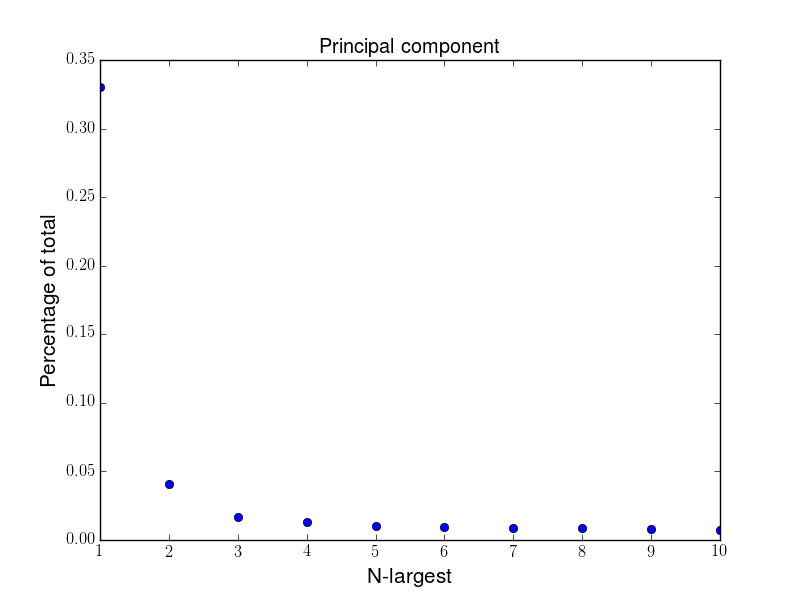
\includegraphics[scale=0.35]{Images/singvals.png}
		\end{center}
		\caption{Percentage of the variance coming from the first ten principal components.}
		\label{singvals}
	\end{figure}
	
	\begin{figure}[H]
		\begin{center}
			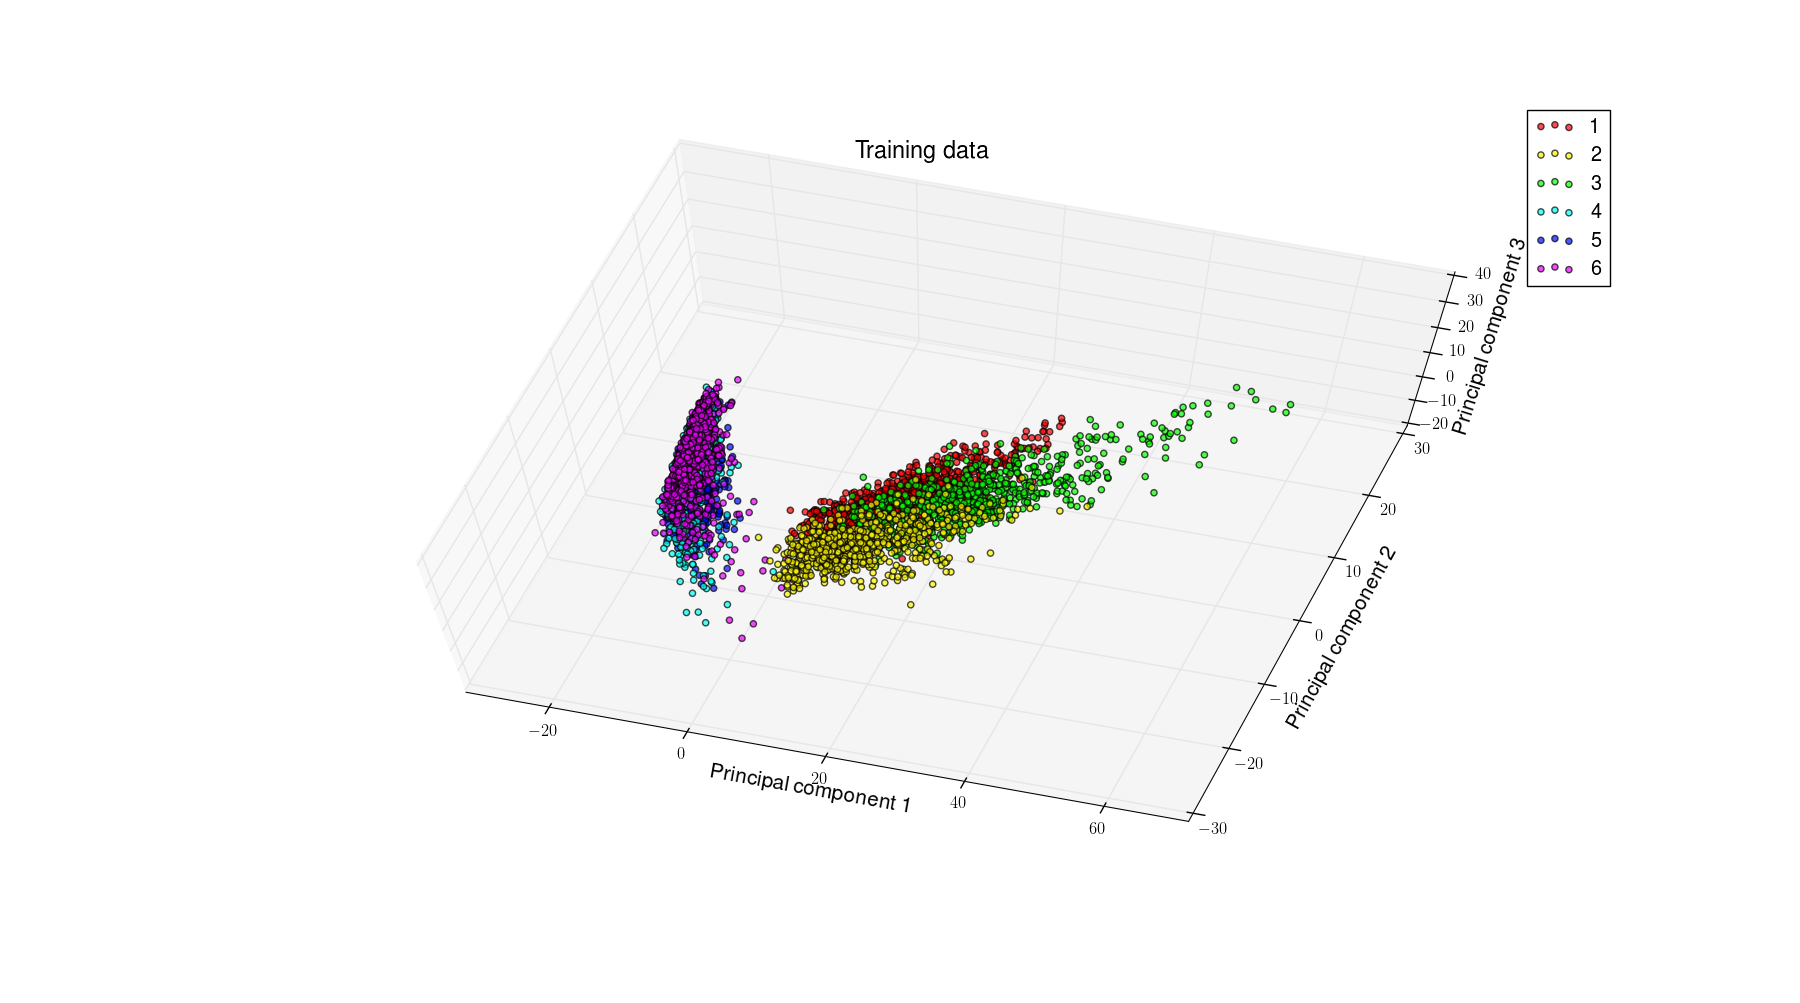
\includegraphics[scale=0.35]{Images/Xtrn.png}
		\end{center}
		\caption{Plot of the training data in the reduced space of the first three principal components}
		\label{Xtrn}
	\end{figure}
	
	\noindent
	We observe firstly that the data corresponding to the active movements seem separable from those of inactive nature. This becomes even more clear in figure \ref{Xactivity}, in which the activity type is plotted instead of the labels of the instances. The labelling of the activity types shown in figure \ref{Xactivity} will be used to distinguish the two and specify which is meant, as it is now known which of the two corresponds to the high (or low) activities. Lastly, the data corresponding to the two activity types have a clearly different shape. It therefore makes sense to plot these separately. In figures \ref{Xtrn1} and \ref{Xtrn2}, these separate plots are shown.
	
	\begin{figure}[H]
		\begin{center}
			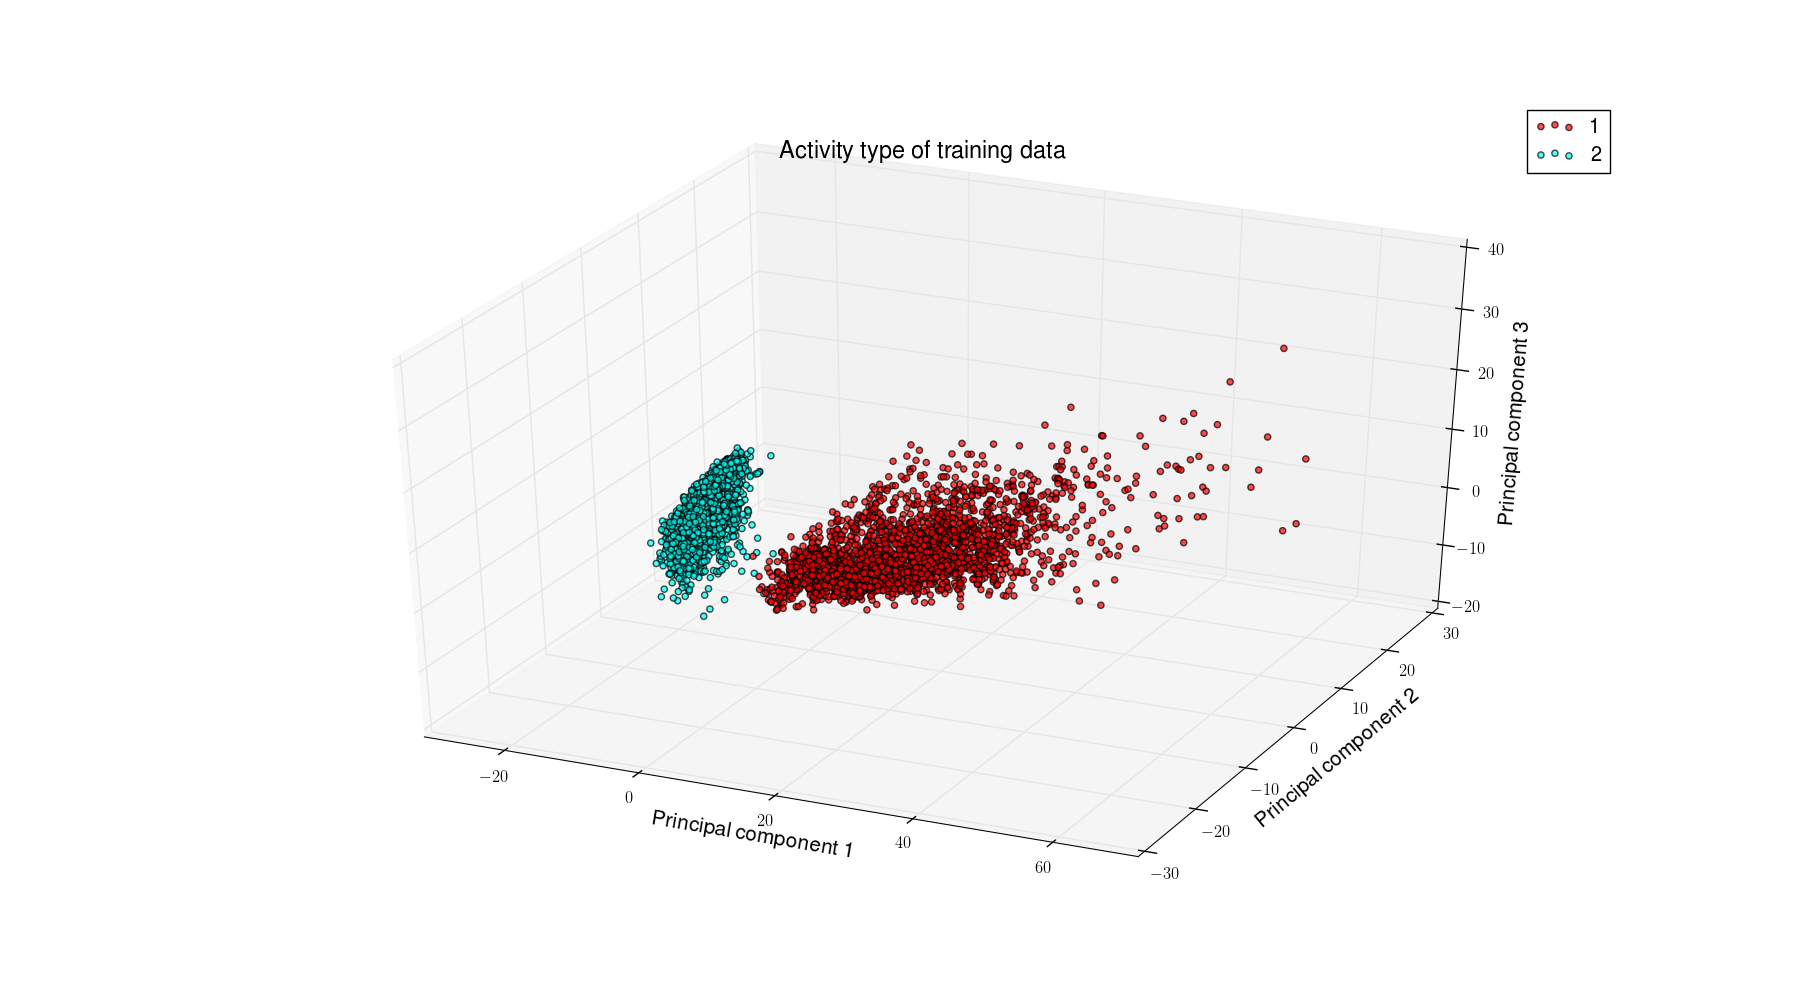
\includegraphics[scale=0.35]{Images/Xactivity.png}
			\caption{Plot of the activity types of the training data}
			\label{Xactivity}
		\end{center}
	\end{figure}
	
	\begin{figure}[H]
		\begin{center}
			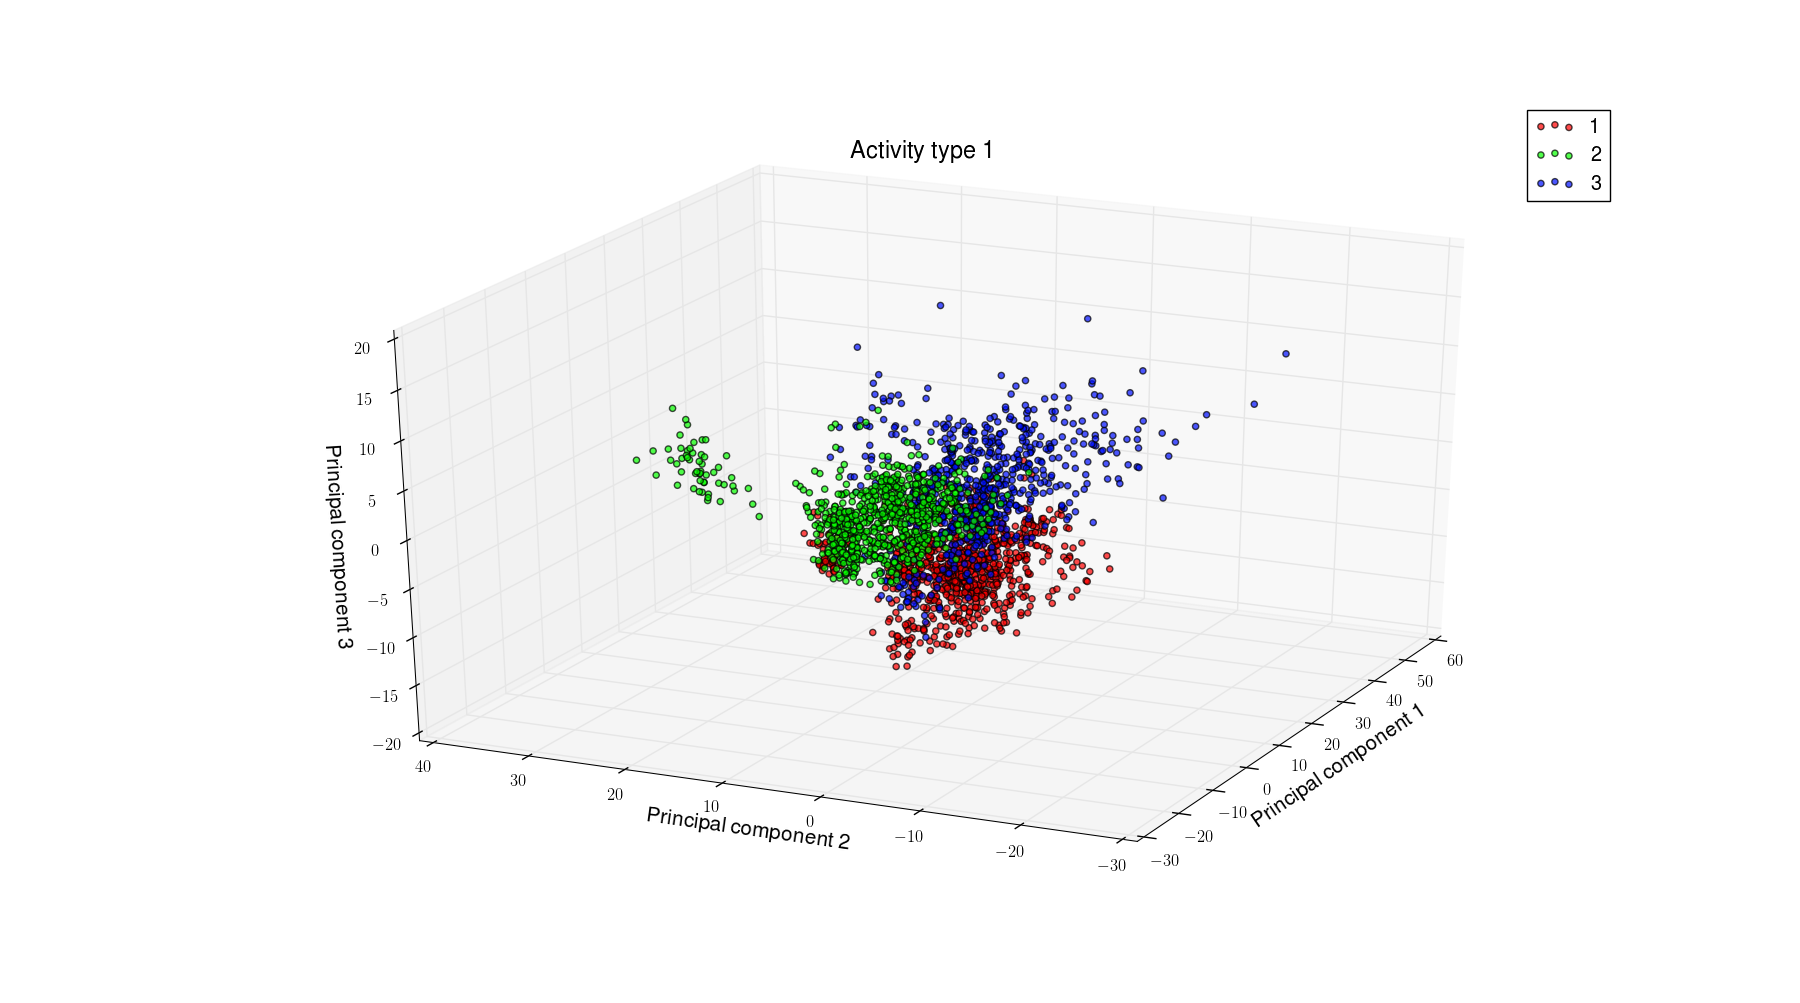
\includegraphics[scale=0.35]{Images/Xtrn1.png}
			\caption{Plot of the training data corresponding to activity type 1 in the reduced space of the first three principal components}
			\label{Xtrn1}
		\end{center}
	\end{figure}
	
	\begin{figure}[H]
		\begin{center}
			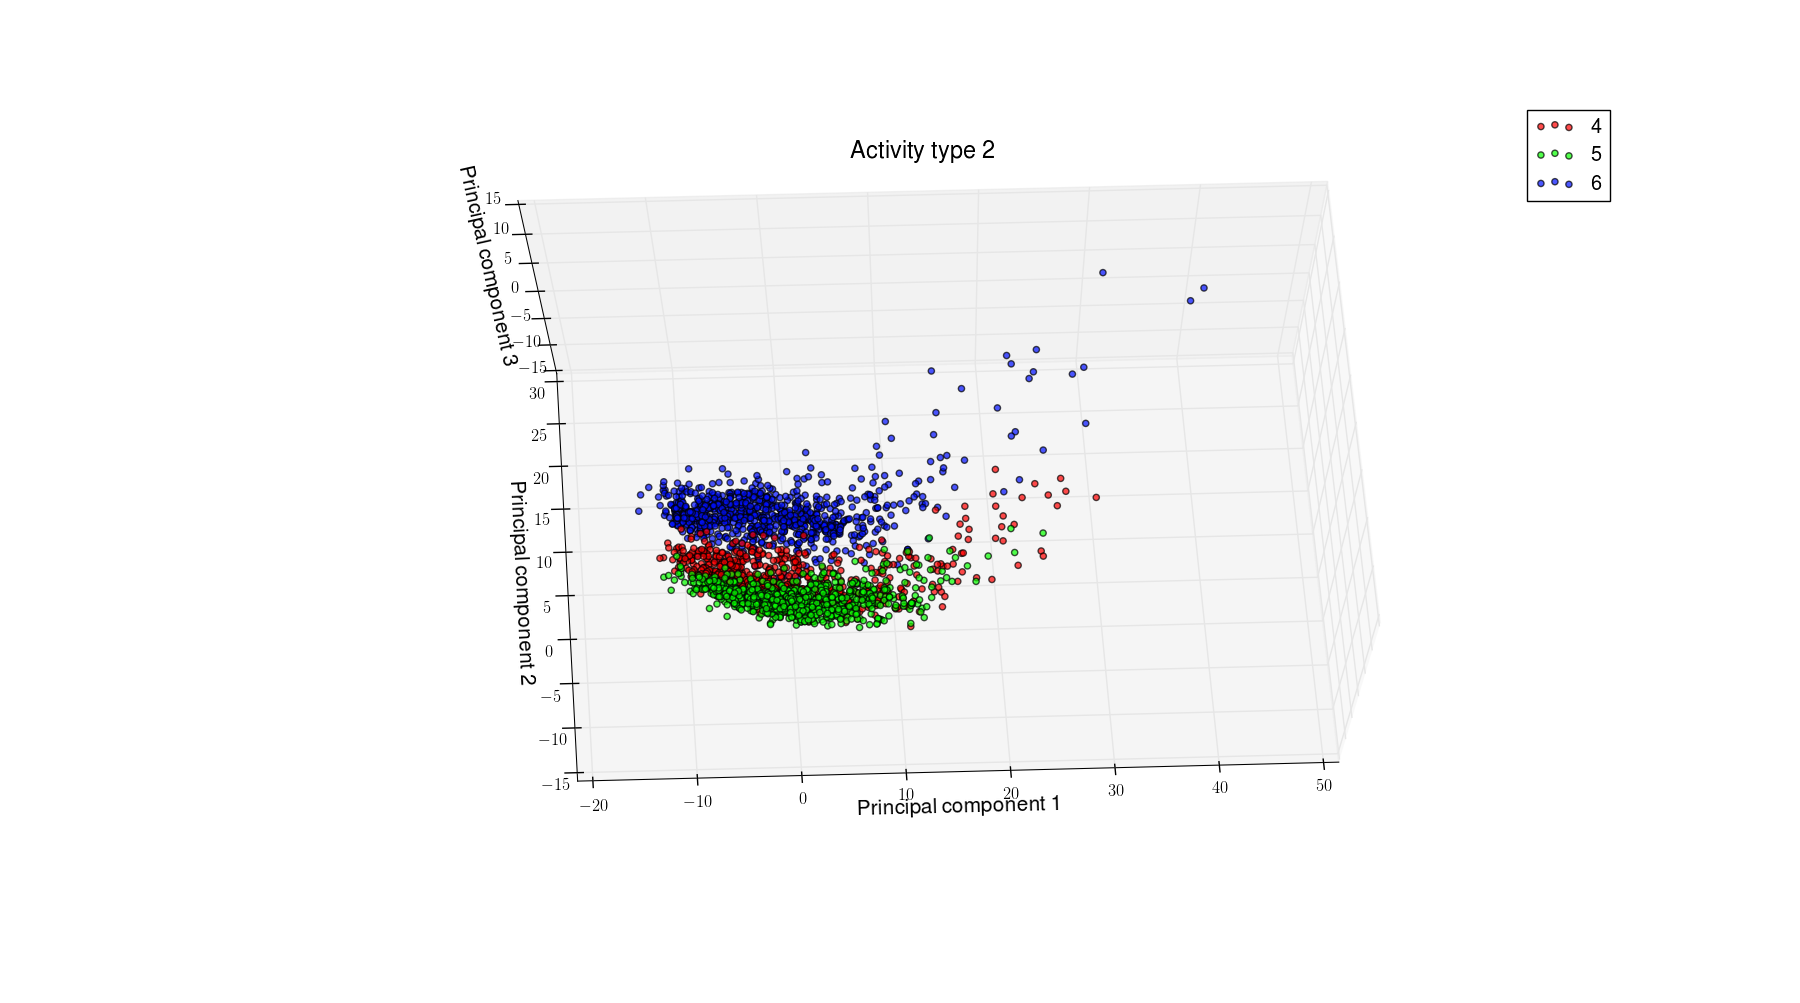
\includegraphics[scale=0.35]{Images/Xtrn2.png}
			\caption{Plot of the training data corresponding to activity type 1 in the reduced space of the first three principal components}
			\label{Xtrn2}
		\end{center}
	\end{figure}
	
	\noindent
	Based on these images, it seems that the labels corresponding to activity type 1 are not completely separable. On the other hand, the ones of activity type 2 seem separably by some non-linear manifold.\\
	
	\noindent
	As the identifiers are also given, the data coming from a single subject for both activity types is shown for a few subjects in figure \ref{subjects}.
	
	\begin{figure}[H]
		\begin{center}
			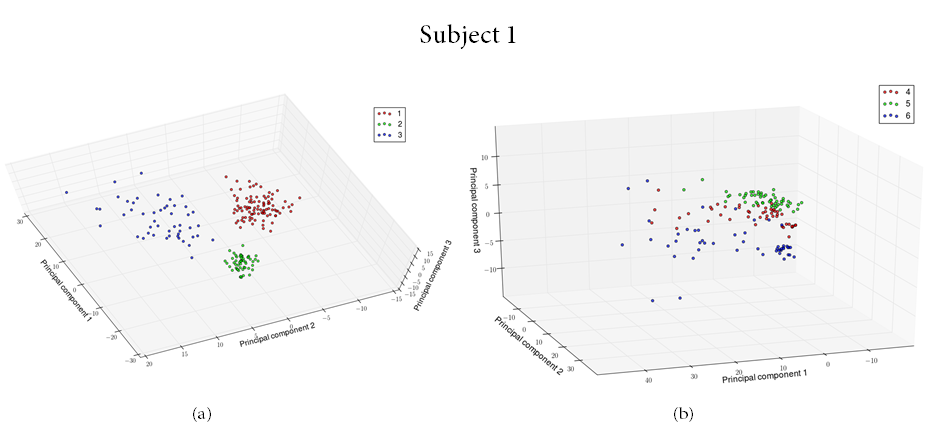
\includegraphics[scale=0.6]{Images/subject1.png}
		\end{center}

		\begin{center}
			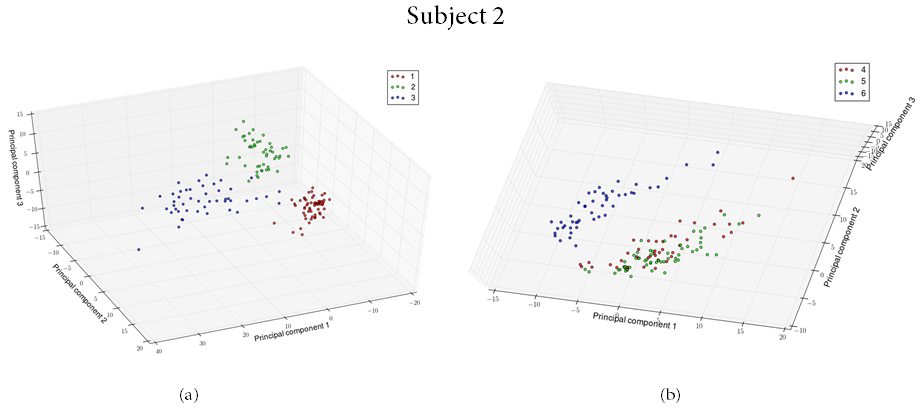
\includegraphics[scale=0.6]{Images/subject2.png}
		\end{center}

		\begin{center}
			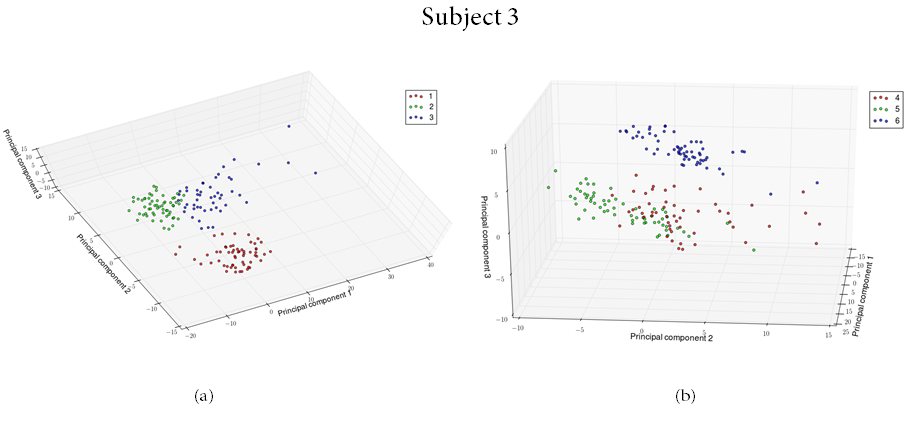
\includegraphics[scale=0.6]{Images/subject3.png}
		\end{center}
		\caption{Plot the data coming from one of the subjects. Both the instances activity type 1 (a) and type 2 (b) are shown.}
		\label{subjects}
	\end{figure}
	
	\noindent
	Firstly, we observe that per subject, the labels of activity type 1 form separate clusters. Secondly, class 6 seems separable from class 4 and 5, but the latter two usually are not. This also corresponds with figure \ref{Xtrn2}. Lastly, it can be seen that the variance of the data coming from different subjects may vary considerably.\\
	
	\noindent
	Finally, we plot both the training and the test set in a single plot in figure \ref{Xall}, as to verify that the training set is representative for the test set. For if this is not the case, one could not expect the classifier trained on the training set to perform well on the test set. Potentially some correction has to be applied, such as in the covariate shift setting. However, in this case it does seem that both datasets are drawn the same distribution, or at least very similar ones. 
	
	\begin{figure}[H]
		\begin{center}
			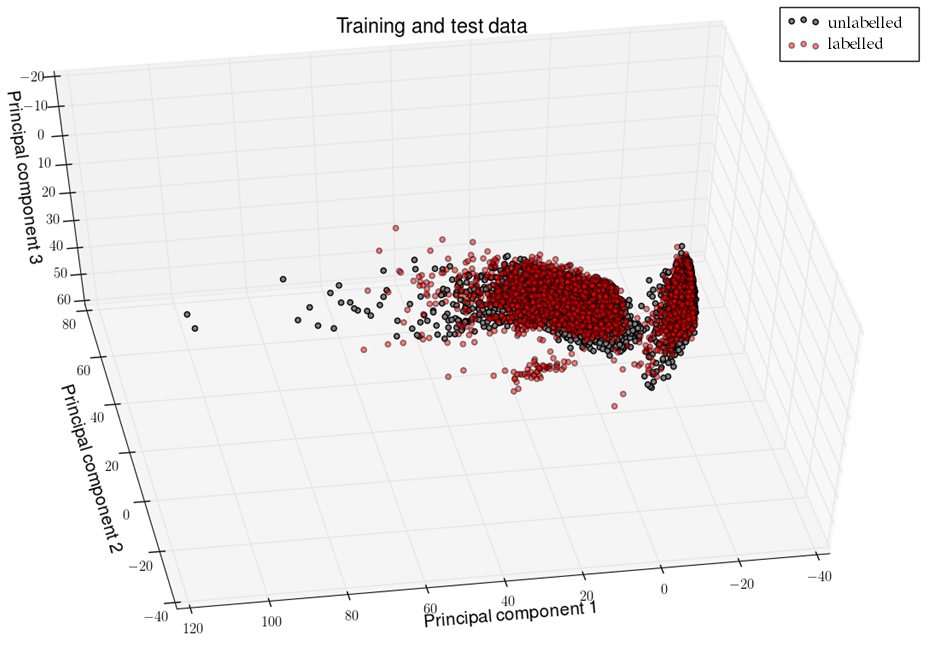
\includegraphics[scale=0.35]{Images/Xall.png}
			\caption{Plot of both the training data (labelled) and the test data (unlabelled).}
			\label{Xall}
		\end{center}
	\end{figure}
	
	
	
	\section*{First try on the training data}
	We next try a few simple
\end{document}